% -*- root: main.tex -*-
%-------------------------------------------------------------------------------
\chapterimage{chapter_head_4.pdf} 

%-------------------------------------------------------------------------------
\chapter{ROS 개념 정리}

%-------------------------------------------------------------------------------
\section{ROS 용어 정리}\index{ROS 용어 정리}\label{sec:RosTerm}

"로봇 운영체제 강좌 : 09. ROS 개념 정리" 강좌에 앞서서 많이 등장하는 ROS 용어들을 골라 정리하였다. ROS 용어 사전처럼 이용하면 좋을 듯 싶고, 보다 더 자세한 설명은 관련 강좌 링크를 추가해 두었다. 이 후의 강좌들을 읽으면서 이해가 안되는 부분이 있으면 참고하도록 하자. 

"로봇 운영체제 강좌 : 08. ROS 용어 정리" / "로봇 운영체제 강좌 : 09. ROS 개념 정리" 강좌는 매우 중요한 개념을 담고 있지만 생소한 용어 사용으로 이해하기 어려울 수 있다. 이 두 강좌를 두 세번 번갈아 보면서 익힐 수 있도록 하고, 이해가 안된다고 포기하지 말고 이해 안되는 부분은 일단 접어두고 다음 강좌로 넘어가서 직접 실전을 통해 익힐 수 있도록 하자.

\begin{definition}[ROS]\label{def:Ros}
로스는 로봇 응용 프로그램을 개발을 위한 운영체제와 같은 로봇 플랫폼이다. 로스는 로봇 응용프로그램을 개발할때 필요한 하드웨어 추상화, 하위 디바이스 제어, 일반적으로 사용되는 기능의 구현, 프로세스간의 메시지 파싱, 패키지 관리, 개발환경에 필요한 라이브러리와 다양한 개발 및 디버깅 도구를 제공한다.
\end{definition}

\begin{definition}[마스터(master)]\label{def:RosMaster}
마스터는 노드와 노드사이의 연결 및 메시지 통신을 위한 네임 서버와 같은 역할을 한다. 로스코어(roscore)가 실행 명령어 이며, 마스터를 실행하게되면 각 노드들의 이름을 등록하고 필요에 따라 정보를 받을 수 있다. 마스터가 없이는 노드간의 접속, 토픽과 서비스와 같은 메시지 통신을 할 수 없다. 

마스터는 마스터에 접속하는 슬레이브들과의 접속 상태를 유지하지 않는 HTTP 기반의 프로토콜인 XMLRPC를 이용하여 슬레이브들과 통신하게 된다. 즉, 슬레이브인 노드들이 필요할때만 접속하여 자신의 정보를 등록하거나 다른 노드의 정보를 요청하여 수신받을 수 있다. 평상시에는 서로간의 접속 상태를 체크하지 않는다. 이러한 기능으로 매우 크고, 복잡한 환경에서도 적용가능하다. 또한, XMLRPC는 매우 가볍고, 다양한 프로그래밍 언어를 지원하고 있기때문에 다기종 하드웨어, 다언어를 지원하는 로스에 매우 적합하다.

로스를 구동하게 되면 사용자가 정해놓은 ROS\_MASTER\_URI 변수에 기재되어 있는 URI 주소 및 포트를 갖는다. 사용자가 설정해놓지 않은 경우에는 URI 주소로 현재의 로컬 IP 를 사용하고, 11311 포트를 이용하게 된다.
\end{definition}

\begin{definition}[노드(node)]\label{def:RosNode}
로스에서 최소 단위의 실행 프로세서를 가르키는 용어이다. 하나의 실행 가능한 프로그램으로 생각하면 된다. 

로스에서는 하나의 목적에 하나의 노드를 작성하길 권하고 있으며 재사용이 쉽도록 구성하여 만들도록 권고하고 있다. 예를들어, 모바일 로봇의 경우, 로봇을 구동하기 위하여 각 프로그램을 세분화 시킨다. 예를들어, 센서 드라이브, 센서 데이타를 이용한 변환, 장애물 판단, 모터 구동, 엔코더 입력, 네이게이션 등 세부화된 작은 노드들을 이용한다.

노드는 생성과 함께 마스터에 노드이름, 발행자이름, 구독자이름, 토픽이름, 서비스이름, 메시지형태, URI 주소 및 포트를 등록한다. 이 정보들을 기반으로 각 노드는 노드끼리 토픽 및 서비스를 이용하여 메시지를 주고 받을 수 있다.

노드는 마스터와 통신할 때, XMLRPC를 이용하며, 노드간의 통신에서는 XMLRPC 및 TCP/IP 통신 계열의 TCPROS를 이용하고 있다. 노드간의 접속 요청 및 응답은  XMLRPC를 사용하며, 메시지 통신은 마스터와는 관계없이 노드와 노드간의 직접적인 통신으로 TCPROS를 이용하고 있다. URI 주소 및 포트는 현재 노드가 실행중인 컴퓨터에 저장된 ROS\_HOSTNAME 라는 환경 변수값을 URI 주소로 사용하며, 포트는 임의적 고유의 값으로 설정되게 된다.  
\end{definition}

\begin{definition}[패키지(package)]\label{def:RosPackage}
로스를 구성하는 기본 단위로써 실행 가능한 노드를 포함하고 있다. 로스는 패키지를 단위로 각각의 응용 프로그램들이 개발된다. 패키지는 최소한 하나 이상의 노드를 포함하고 있다. ROS Hydro의 경우 공식적으로 약 700개 의 패키지를 제공하고 있으며, 유저들이 개발하여 공개된 패키지가 대략 3300개에 달하고 있다. 
\end{definition}

\begin{definition}[메타패키지(metapackage)]\label{def:RosMetapackage}
공통된 목적을 가지는 패키지들을 모아둔 패키지들의 집합을 말한다. 복수의 패키지를 포함하고 있다.
\end{definition}

\begin{definition}[메시지(message,msg)]\label{def:RosMessage}
노드는 메시지를 통해 노드간의 데이터를 주고받게 된다. 메시지는 integer, floating point, boolean 와 같은 변수형태이다. 또한, 메시지안에 메시지를 품고 있는 간단한 데이터 구조 및 메시지들의 배열과 같은 구조도 사용할 수 있다. 

메세지를 이용한 통신방법으로는 TCPROS, UDPROS 방식등이 있으며, 단방향 메시지 송/수신 방식의 토픽과 양방향 메시지 요청/응답 방식의 서비스를 이용하고 있다.
\end{definition}

\begin{definition}[토픽(topic)]\label{def:RosTopic}
토픽은 "이야깃거리"이다. 발행자 노드가 하나의 이야깃거리에서 대해서 토픽이라는 이름으로 마스터에 등록한 후, 이야깃거리에 대한 이야기를 메시지 형태로 발행한다. 이 이야깃거리를 수신 받기를 원하는 구독자 노드는 마스터에 등록된 토픽의 이름에 해당되는 발행자 노드의 정보를 받는다. 이 정보를 기반으로 구독자 노드는 발행자 노드와 직접적으로 연결하여 메시지를 송/수신 또는 요청/응답 받게 된다. 
\end{definition}

\begin{definition}[발행(publish) 및 발행자(Publisher) ]\label{def:RosPublish}
발행은 토픽의 내용에 해당되는 메시지 형태의 데이터를 송신하는 것을 말한다. 

발행자 노드는 발행을 수행하기 위하여 토픽을 포함한 자신의 정보들을 마스터에 등록하고, 구독을 원하는 구독자 노드에게 메시지를 보내게 된다. 발행자는 이를 실행하는 개체로써 노드에서 선언하게 된다. 발행자는 하나의 노드에서 복수로 선언이 가능하다.
\end{definition}

\begin{definition}[구독(subscribe) 및 구독자(Subscriber)]\label{def:RosSubscribe}
구독은 토픽의 내용에 해당되는 메시지 형태의 데이터를 수신하는 것을 말한다. 

구독자 노드는 구독을 수행하기 위하여 토픽을 포함한 자신의 정보들을 마스터에 등록하고, 구독하고자 하는 토픽을 발행하는 발행자 노드의 정보를 마스터로부터 받는다. 이 정보를 기반으로 구독자 노드는 발행자 노드와 직접적으로 접속하여 발행자 노드로부터 메시지를 받게 된다. 구독자는 이를 실행하는 개체로써 노드에서 선언하게 된다. 구독자는 하나의 노드에서 복수로 선언이 가능하다.
\end{definition}

\begin{definition}[서비스(service)]\label{def:RosService}
발행과 구독 개념의 토픽 통신 방식은 비동기 방식이라 필요에 따라서 주어진 데이터를 전송하고 받기에 매우 훌륭한 방법이다. 또한, 한번의 접속으로 지속적인 메시지를 송/수신하기 때문에 지속적으로 메시지를 발송해야하는 센서 데이터에 적합하여 많이 사용되고 있다. 

하지만, 경우에 따라서는 요청과 응답이 함께 사용되는 동기 방식의 메시지 교환 방식도 필요하다. 이에따라, 로스에서는 서비스라는 이름으로 메시지 동기 방식을 제공하고 있다. 

서비스는 요청이 있을 경우에 응답을 하는 서비스 서버와 요청을 하고 응답을 받는 서비스 클라이언트로 나뉘어 있다. 서비스는 토픽과는 달리 1회성 메시지 통신이다. 서비스의 요청과 응답이 완료되면 연결된 두 노드의 접속은 끊기게 된다. 
\end{definition}

\begin{definition}[서비스 서버 (service server)]\label{def:RosServiceServer}
서비스 서버는 요청을 입력으로 받고, 응답을 출력으로 하는 서비스 메시지 통신의 서버 역할을 말한다. 요청과 응답은 모두 메시지로 되어 있으며, 서비스 요청에 의하여 주어진 서비스를 수행 후에 그 결과를 서비스 클라이언트에게 전달한다. 서비스 메시지 방식은 동기식이기에 정해진 명령을 지시 및 수행하는 노드에 사용하는 경우가 많다.
\end{definition}

\begin{definition}[서비스 클라이언트 (service client)]\label{def:RosServiceClient}
서비스 클라이언트는 요청을 출력으로 하고, 응답을 입력으로 받는 서비스 메시지 통신의 클라이언트 역할을 말한다. 요청과 응답은 모두 메시지로 되어 있으며, 서비스 요청을 서비스 서버에 전달하고 그 결과 값을 서비스 서버로 부터 받는다. 서비스 메시지 방식은 동기식이기에 정해진 명령을 지시 및 수행하는 노드에 사용하는 경우가 많다.
\end{definition}

\begin{definition}[캐킨(catkin)]\label{def:RosCatkin}
로스의 빌드 시스템을 말한다. 로스의 빌드 시스템은 기본적으로 CMake(Cross Platform Make) 를 이용하고 있어서 패키지 폴더에 CMakeLists.txt 라는 파일에 빌드 환경을 기술하고 있다. 로스에서는 CMake 를 로스에 맞도록 수정하여 로스에 특화된 캐킨 빌드 시스템을 만들었다. 캐킨 빌드 시스템은 로스와 관련된 빌드, 패키지 관리, 패키지간의 의존관계 등을 편리하게 사용할 수 있도록 하고 있다. 
\end{definition}

\begin{definition}[로스빌드(rosbuild)]\label{def:RosRosbuild}
catkin 빌드 시스템의 이전에 사용되었던 빌드 시스템이다. ROS Fuerte 버전부터 rosbuild 빌드 시스템 대신에 catkin 빌드 시스템을 사용하고 있으나, rosbuild 빌드 시스템 또한 사용가능하다. 하지만, 이는 ROS 버전의 호환성을 위해 남겨둔 것이지 공식적으로는 추천하지 않는다. 만약, rosbuild 빌드 시스템을 사용한 이전 패키지를 사용해야만 한다면 rosbuild를 catkin으로 변경하여 사용하기를 추천한다. 
\end{definition}

\begin{definition}[로스코어(roscore)]\label{def:RosCore}
로스 마스터를 구동하는 명령어이다. 같은 네트웍이라면 다른 컴퓨터에서 실행하여도 된다. 로스를 구동하게 되면 사용자가 정해놓은 ROS\_MASTER\_URI 변수에 기재되어 있는 URI 주소 및 포트를 갖는다. 사용자가 설정해놓지 않은 경우에는 URI 주소로 현재의 로컬 IP 를 사용하고, 11311 포트를 이용하게 된다.
\end{definition}

\begin{definition}[매개변수(parameter)]\label{def:RosParameter}
노드에서 사용되는 매개변수를 말한다. 흔히, 윈도우즈 프로그램에서 *.ini 설정파일과 같다고 생각하면 된다. 디폴트로 설정 값들이 지정되어 있고, 필요에 의해서 외부에서 이 매개변수를 읽기, 쓰기가 가능하다. 특히, 상황에 맞추어 이 매개변수를 외부에서 쓰기기능을 이용하여 설정값을 실시간으로 바꿀수 있기에 매우 유용한 방법이다. 예를들어 접속하는 USB포트 및 카메라 캘리브레이션 값, 속도 및 명령어들의 최대/최저 값 등의 설정등을 지정할 수 있다.
\end{definition}

\begin{definition}[매개변수 서버(parameter server)]\label{def:RosParameterServer}
매개변수 서버는 패키지에서 매개변수를 사용할 때, 각 매개변수를 등록하는 서버를 말한다. 매개변수 서버는 마스터의 일부분이다. 
\end{definition}

\begin{definition}[rosrun]\label{def:RosRun}
로스의 기본적인 실행 명령어이다. 패키지에서 하나의 노드를 실행하는데 사용된다. 노드가 사용하는 URI 주소 및 포트는 현재 노드가 실행중인 컴퓨터에 저장된 ROS\_HOSTNAME 라는 환경 변수값을 URI 주소로 사용하며, 포트는 임의적 고유의 값으로 설정되게 된다.
\end{definition}

\begin{definition}[roslaunch]\label{def:RosLaunch}
로스런(rosrun)이 하나의 노드를 실행하는 명령어라면 로스런치(roslaunch)는 복 수개의 노드를 실행하는 개념이다. 이 명령어를 통해 정해진 단일 혹은 복수의 노드를 실행시킬 수 있다. 

그 이외의 기능으로 실행시에 패키지의 매개변수를 변경, 노드 명의 변경, 노드 네임 스페이스 설정, ROS\_ROOT 및 ROS\_PACKAGE\_PATH 설정, 이름 변경, 환경 변수 변경 등의 실행시 변경할 수 있는 많은 옵션들을 갖춘 노드 실행에 특화된 로스 명령어이다. 

로스런치는 "*.launch" 라는 로스런치파일을 사용하여 실행 노드에 대한 설정을 해주는데 이는 XML 기반으로 되어 있으며, 태그별 옵션을 제공하고 있다. 실행 명령어로는 "roslaunch 패키지명 로스런치파일" 이다.
\end{definition}

\begin{definition}[배그(bag)]\label{def:RosBag}
로스에서 주고받는 메시지의 데이터를 저장할 수 있는 있는데 이를 배그라고 한다. ROS에서는 이 배그를 이용하여 메시지를 저장하고 필요로 할 때 이를 재생하여 이전 상황을 그대로 재현할 수있는 기능을 갖추고 있다. 예를들어, 센서를 이용한 로봇 실험을 실행할 때, 센서 값을 배그를 이용하여 메시지 형태로 저장한다. 이 저장된 메시지는 같은 실험을 수행하지 않아도 저장해둔 배그 파일을 재생하는 것으로 그 당시의 센서값을 반복 사용가능하다. 특히, 기록, 재생의 기능을 활용하여 반복되는 프로그램 수정이 많은 알고리즘 개발에 매우 유용하다. 
\end{definition}

\begin{definition}[ros wiki]\label{def:RosWiki}
로스의 각 패키지 및 기능들을 설명하는 페이지(http://wiki.ros.org/)이다.  각 패키지는 위키 패이지를 가지고 있어서 패키지에 대한 간단한 설명, 사용되는 매개변수, 저작자, 라이선스, 홈페이지, 저장소, 튜토리얼등을 포함하고 있다.
\end{definition}

\begin{definition}[저장소(repositoy)]\label{def:RosRepository}
공개된 패키지의 경우, 각 패키지의 위키에 저장소를 명시하고 있다. 저장소는 패키지가 저장된 웹상의 저장소 URL 주소이며 svn, hg, git 등의 소스 관리 시스템을 이용하여 이슈, 개발, 다운로드 등을 관리하고 있다.
\end{definition}

\begin{definition}[그래프(graph)]\label{def:RosGraph}
위에서 설명한 노드, 토픽, 발행자, 구독자 관계를 그래프를 통해 나타나게 하는 것이다. 현재 실행중인 메시지 통신을 그래프화 시킨 것으로 1회성인 서비스에 대한 그래프는 작성할 수 없다. 실행은 rqt\_graph 패키지의 rqt\_graph 노드를 실행하면 된다. "rqt\_graph" 또는 "rosrun rqt\_graph rqt\_graph" 명령어를 이용하면 된다.   
\end{definition}

\begin{definition}[이름(name)]\label{def:RosName}
노드, 매개변수, 토픽, 서비스는 모두 이름을 갖고 있다. 이 이름은 마스터에 등록하고 각 노드의 매개변수, 토픽, 서비스를 사용할때 이 이름을 기반으로 상호적으로 동작하도록 되어있다. 또한, 이름은 실행시에 변경가능하기 때문에 매우 유연하고, 같은 노드, 매개변수, 토픽, 서비스라고 하여도 다른 이름으로 중복 실행이 가능하다. 이러한 이름의 사용으로 로스는 큰 규모의 프로젝트, 복잡한 구조의 시스템에도 적합하다.  
\end{definition}

\begin{definition}[클라이언트 라이브러리(client libray)]\label{def:RosClientLibray}
로스는 사용되는 언어의 의존성을 낮추기 위하여 클라이언트 라이브러리라는 이름으로 각종 언어의 개발환경을 제공하고 있다. 

주요한 클라이언트 라이브러리로는 C++, Python, Lisp 등이 있으며, 그 이외에도 java, lua, .NET, EusLisp, R 등의 언어들을 사용가능하다. 이를 위해 roscpp, rospy, roslisp, rosjava, roslua, roscs, roseus, PhaROS, rosR 등의 클라이언트 라이브러리가 개발되었다.
\end{definition}

\begin{definition}[URI (Uniform Resource Identifier)]\label{def:RosURI}
URI (Uniform Resource Identifier, 통합 자원 식별자) 는 인터넷에 있는 자원을 나타내는 유일한 주소이다. URI 은 인터넷에서 요구되는 기본조건으로서 인터넷 프로토콜에서 식별자로 사용된다.
\end{definition}

\begin{definition}[MD5 (Message-Digest algorithm 5)]\label{def:RosMD5}
MD5는 128비트 암호화 해시 함수이다. 주로 프로그램이나 파일이 원본 그대로인지를 확인하는 무결성 검사 등에 사용된다. 로스에서의 메시지를 이용한 통신에서 MD5를 이용하여 메시지 송수신의 무결성 검사를 하고 있다.
\end{definition}

\begin{definition}[RPC(Remote Procedure Call)]\label{def:RosRPC}
RPC란 '멀리 떨어져(Remote) 있는 컴퓨터상의 프로그램이 다른 컴퓨터 내에 있는 서브프로그램(Procedure)을 불러내는(Call)' 것을 의미한다. 컴퓨터 프로그램이 다른 주소 공간에서 원격 제어를 위한 프로그래머의 세세한 코딩 없이 함수나 프로시저의 실행을 허용하는 기술로써 대표적으로는 TCP/IP, IPX 등의 전송 프로토콜을 이용한다. 
\end{definition}

\begin{definition}[XML(Extensible Markup Language)]\label{def:RosXML}
XML은 W3C에서 다른 특수 목적의 마크업 언어를 만드는 용도에서 권장되는 다목적 마크업 언어(markup language)로 태그 등을 이용하여 데이터의 구조를 명기하는 언어의 한 가지이다. 
\end{definition}

\begin{definition}[XMLRPC]\label{def:RosXMLRPC}
XML-RPC란, RPC 프로토콜의 일종으로서, 인코딩 형식에서는 XML을 채택하고, 전송 방식에서는 접속 상태를 유지하지 않고 체크하지 않는 요청/응답 방식의 HTTP 프로토콜을 사용하고 있다. XML-RPC는 매우 단순한 규약으로서, 작은 데이터 형식이나 명령을 정의하는 정도로만 사용하고 있어서 꽤나 단순한 편이다. 이러한 특징으로, XMLRPC는 매우 가볍고, 다양한 프로그래밍 언어를 지원하고 있기 때문에 다기종 하드웨어, 다언어를 지원하는 로스에 매우 적합하다.
\end{definition}

\begin{definition}[TCP/IP (Transmission Control Protocol / Internet Protocol)]\label{def:RosTCPIP}
TCP 는 Transmission Control Protocol 의 약자로써, 전송 제어 프로토콜이라고 부른다. 흔히 TCP/IP 라 부르는데 이는 인터넷 프로토콜 계층의 시각에서 보면 IP(Internet Protocol) 를 기반으로 전송 제어 프로토콜인 TCP 를 사용하여 데이터의 전달을 보증하고 보낸 순서대로 송/수신하게 된다. 
\end{definition}

\begin{definition}[TCPROS]\label{def:RosTCPROS}
메시지 및 서비스에서 사용되는 TCP/IP 기반의 메시지 방식을 TCPROS라고 한다.
\end{definition}

\begin{definition}[UDPROS]\label{def:RosUDPROS}
메시지 및 서비스에서 사용되는 UDP 기반의 메시지 방식을 UDPROS라고 한다. 일반적으로 ROS에서는 사용되지 않고 있다.
\end{definition}

\begin{definition}[CMakeLists.txt]\label{def:RosCMakeLists.txt}
로스의 빌드 시스템인 캐킨은 기본적으로 CMake를 이용하고 있어서 패키지 폴더에 CMakeLists.txt 라는 파일에 빌드 환경을 기술하고 있다.
\end{definition}

\begin{definition}[package.xml]\label{def:RosPackage.XML}
패키지의 정보를 담은 XML 파일로써 패키지의 이름, 저작자, 라이선스, 의존성 패키지 등을 기술하고 있다.
\end{definition}

%-------------------------------------------------------------------------------
\section{ROS 개념 정리}\index{ROS 개념 정리}

%-------------------------------------------------------------------------------
\subsection{메시지 통신}\index{메시지 통신}

지금까지 로스에 대해서 설명하였지만, 실제로 어떻게 동작하는 것인지에 대해서는 자세히 언급하지 않았었다. 이번 강좌에서는 로스의 동작에 대한 핵심 기능 및 개념에 대해서 설명하려고 한다. 로스는 매우 생소한 용어들이 많이 등장하므로 "ROS 강좌 : 08. ROS 용어 정리"를 참고하면서 로스 개념을 이해하면 좋을 듯 싶다. 로스 개념 설명에서 사용되는 각 용어들의 상세한 설명은 용어 정리 강좌를 참조하기 바라며, 이번 강좌에서는 개념만을 설명하도록 하겠다.

로스의 핵심 개념은 노드간의 메시지 통신\footnote{ROS Wiki,"Concepts", http://wiki.ros.org/ROS/Concepts}\footnote{ROS Wiki,"Higher-Level Concepts", http://wiki.ros.org/ROS/Higher-Level\%20Concepts}이다. 목적에 따라 세분화된 최소 단위의 실행 프로그램인 노드는 다른 노드와 처리 결과 값을 주고 받게 됨으로써 하나의 커다란 프로그램이 된다. 이를 위하여 메시지 통신에는 단 방향으로 연속적으로 메시지를 송수신하는 토픽 메시지 통신과 쌍 방향으로 요청과 응답 형태의 정해진 작업을 수행하게 하는 목적의 서비스 메시지 통신이 있다. 

이러한 노드간의 메시지 통신에는 접속이 필요한데, 노드간의 접속을 돕는 것이 마스터\footnote{ROS Wiki,"Master", http://wiki.ros.org/Master}이다. 마스터는 노드의 이름, 토픽 및 서비스의 이름, URI 주소와 포트, 매개변수 등의 네임 서버와 같은 역할을 하게된다. 즉, 노드는 생성과 동시에 마스터에 자신의 정보를 등록하게 되고, 다른 노드가 마스터를 통해 접속하려는 노드의 정보를 마스터로부터 취득한다. 그 후, 노드와 노드가 직접 접속하여 메시지 통신을 하는 것이다. 

이를 그림으로 나태내면 다음의 그림과 같다. 마스터는 노드들의 정보를 관리하며, 각 노드는 필요에 따라 다른 노드와 접속, 메시지 통신을 하게 된다. 여기서 우리는 가장 중요한 마스터, 노드, 토픽\footnote{ROS Wiki,"Topics", http://wiki.ros.org/Topics}, 서비스\footnote{ROS Wiki,"Services", http://wiki.ros.org/Services}, 메시지\footnote{ROS Wiki,"Messages", http://wiki.ros.org/Messages}의 흐름에 대해서 알아보도록 하자.

\begin{figure}[h]
\centering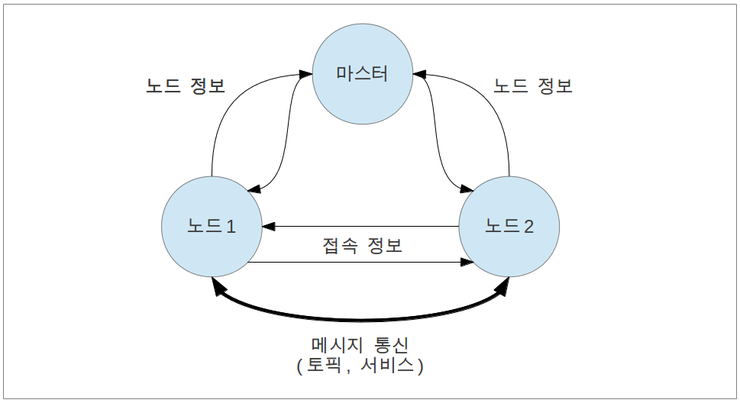
\includegraphics[width=0.6\columnwidth]{pictures/chapter4/message_communication.png}
\caption{메시지 통신}
\end{figure}


%-------------------------------------------------------------------------------
\subsection{마스터 구동}\index{마스터 구동}

노드들간의 메시지 통신에서 연결 정보를 관리하는 마스터는 로스를 사용하기 위해서 제일 먼저 구동해야하는 필수 요소이다. 다음과 같이 "roscore"라는 실행 명령어로 로스 마스터는 구동되며, XMLRPC으로 서버를 구동하게 된다. 마스터는 노드간의 접속을 위하여 노드들의 이름, 토픽 및 서비스의 이름, 메시지 형태, URI 주소 및 포트를  등록받고, 요청이 있을 경우 이 정보를 다른 노드에게 알려주는 역할을 한다.

\begin{lstlisting}[language=bash]
roscore
\end{lstlisting}

\begin{figure}[h]
\centering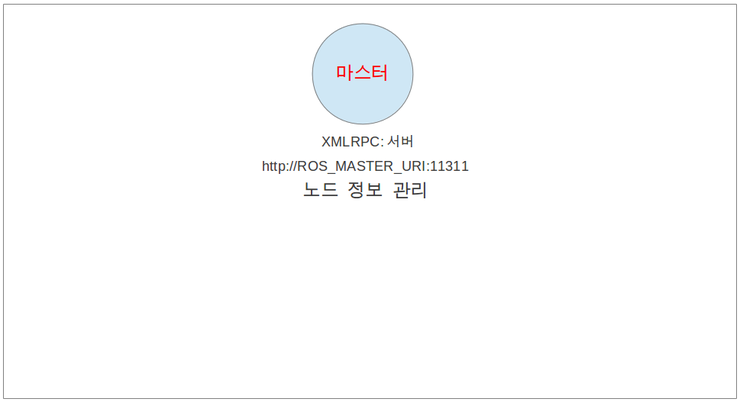
\includegraphics[width=0.6\columnwidth]{pictures/chapter4/notion1.png}
\caption{마스터 구동}
\end{figure}

%-------------------------------------------------------------------------------
\subsection{구독자 노드(Node) 구동}\index{구독자 노드(Node) 구동}
 
구독자 노드는 다음과 같이  "rosrun" 및 "roslaunch" 라는 실행 명령어로 구동된다. 구독자 노드는 구동과 함께 마스터에 자신의 구독자노드이름, 토픽이름, 메시지형태, URI 주소 및 포트를 등록한다. 마스터와 노드는 XMLRPC 를 이용하여 통신하게 된다.

\begin{lstlisting}[language=bash]
rosrun PACKAGE_NAME NODE_NAME
\end{lstlisting}

\begin{lstlisting}[language=bash]
roslaunch PACKAGE_NAME LAUNCH_NAME
\end{lstlisting}

\begin{figure}[h]
\centering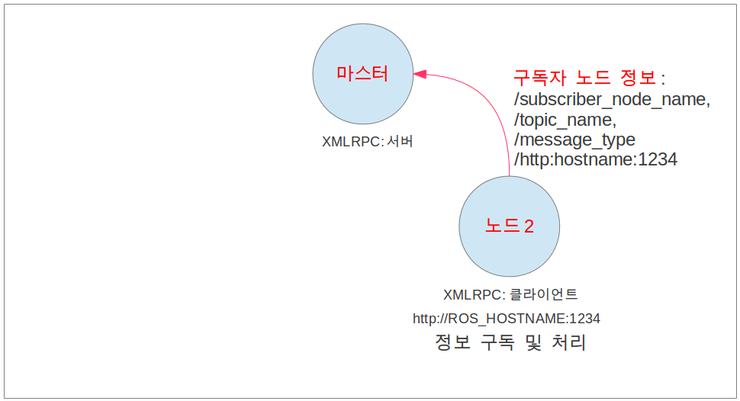
\includegraphics[width=0.6\columnwidth]{pictures/chapter4/notion2.png}
\caption{구독자 노드 구동}
\end{figure}

%-------------------------------------------------------------------------------
\subsection{발행자 노드(Node) 구동}\index{발행자 노드(Node) 구동}

발행자 노드는 구독자 노드와 마찬가지로 "rosrun" 및 "roslaunch" 라는 실행 명령어로 구동한다. 발행자 노드는 구동과 함께 마스터에 자신의 발행자노드이름, 토픽이름, 메시지형태, URI 주소 및 포트를 등록한다. 마스터와 노드는 XMLRPC 를 이용하여 통신하게 된다.

\begin{figure}[h]
\centering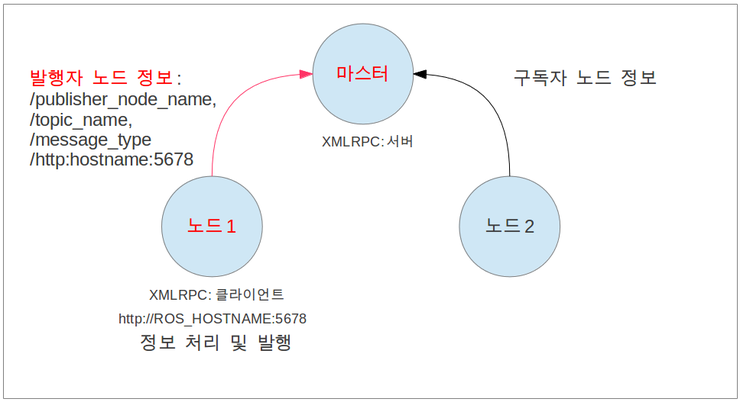
\includegraphics[width=0.6\columnwidth]{pictures/chapter4/notion3.png}
\caption{발행자 노드 구동}
\end{figure}

%-------------------------------------------------------------------------------
\subsection{발행자 정보 알림}\index{발행자 정보 알림}

마스터는 구독자 노드에게 새로운 발행자 정보를 알린다. 마스터와 노드는 XMLRPC 를 이용하여 통신하게 된다.

\begin{figure}[h]
\centering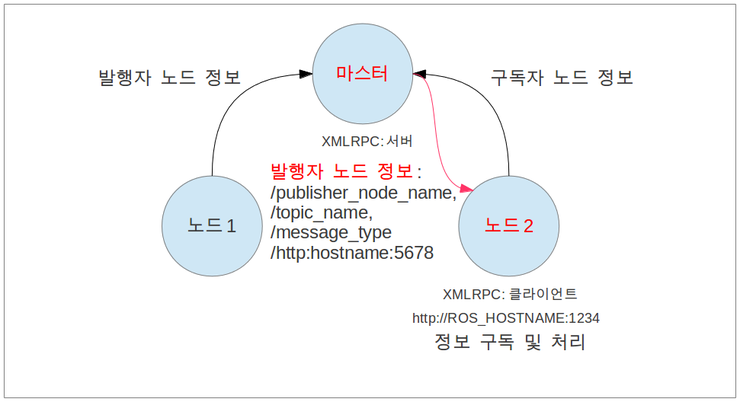
\includegraphics[width=0.6\columnwidth]{pictures/chapter4/notion4.png}
\caption{발행자 정보 알림}
\end{figure}

%-------------------------------------------------------------------------------
\subsection{발행자 노드에 접속 요청}\index{발행자 노드에 접속 요청}

구독자 노드는 마스터로부터 받은 발행자 정보를 기반으로 발행자 노드에게 직접 접속 요청을 한다. 이때에 전송하는 정보로는 자신의 구독자 노드 이름, 토픽이름, 메시지방식(TCPROS 또는 UDPROS)이 있다. 발행자 노드와 구독자 노드는 XMLRPC 를 이용하여 통신하게 된다.

\begin{figure}[h]
\centering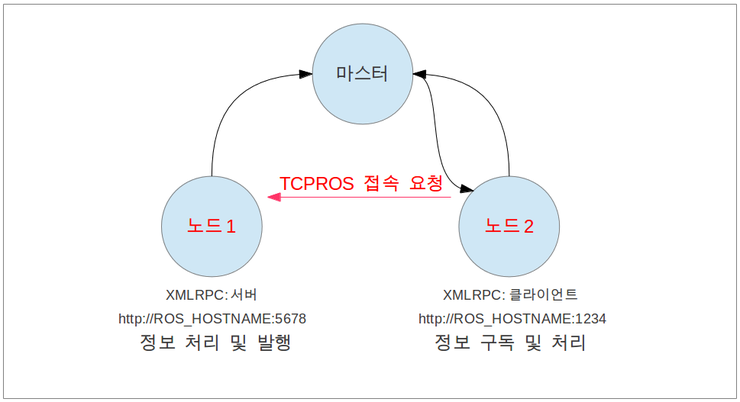
\includegraphics[width=0.6\columnwidth]{pictures/chapter4/notion5.png}
\caption{발행자 노드에 접속 요청}
\end{figure}

%-------------------------------------------------------------------------------
\subsection{발행자 노드에 접속 응답}\index{발행자 노드에 접속 응답}

발행자 노드는 구독자노드에게 접속 응답에 해당되는 자신의 TCP 서버의 정보인 URI주소와 포트를 전송한다. 발행자 노드와 구독자 노드는 XMLRPC 를 이용하여 통신하게 된다.

\begin{figure}[h]
\centering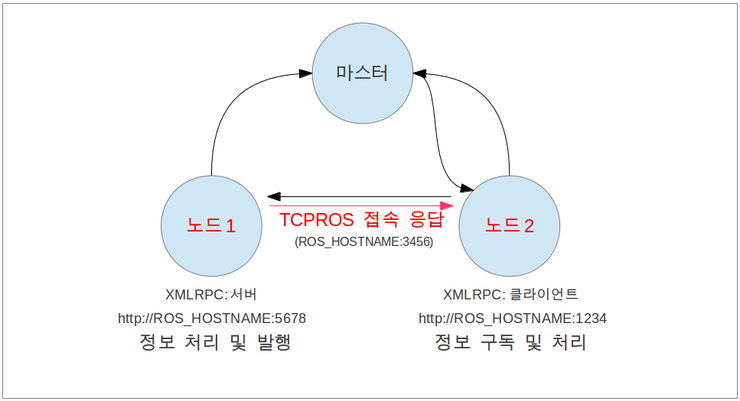
\includegraphics[width=0.6\columnwidth]{pictures/chapter4/notion6.png}
\caption{발행자 노드에 접속 응답}
\end{figure}

%-------------------------------------------------------------------------------
\subsection{TCP 접속}\index{TCP 접속}

구독자 노드는 TCPROS를 이용하여 발행자노드에 대한 클라이언트를 만들고, 발행자노드와 직접 연결한다. (노드간의 통신 방식으로는 TCPROS라 하는 TCP/IP 방식을 이용한다.)

\begin{figure}[h]
\centering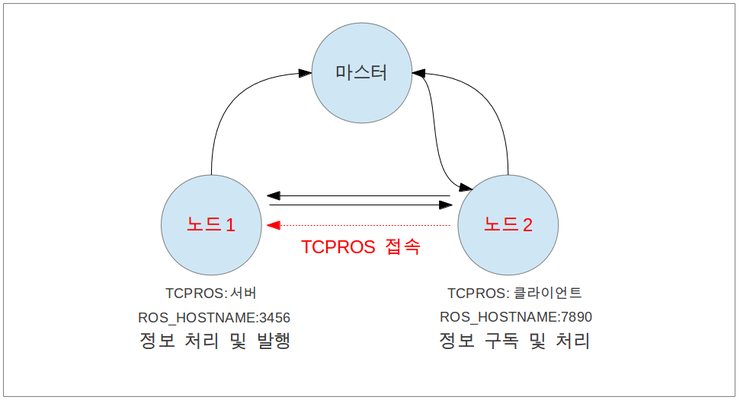
\includegraphics[width=0.6\columnwidth]{pictures/chapter4/notion7.png}
\caption{TCP 접속}
\end{figure}

%-------------------------------------------------------------------------------
\subsection{메시지 전송}\index{메시지 전송}

발행자 노드는 구독자 노드에게 정해진 메시지를 전송한다. (노드간의 통신 방식으로는 TCPROS라 하는 TCP/IP 방식을 이용한다.)

\begin{figure}[h]
\centering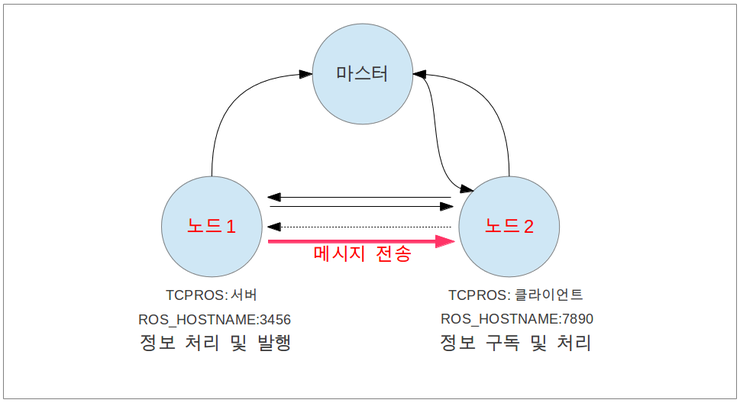
\includegraphics[width=0.6\columnwidth]{pictures/chapter4/notion8.png}
\caption{메시지 전송}
\end{figure}

%-------------------------------------------------------------------------------
\subsection{서비스 요청 및 응답}\index{서비스 요청 및 응답}

위에서 설명한 내용은 메시지 통신중에 토픽에 해당된다. 토픽의 경우, 발행자 및 구독자가 중지하지 않는 이상, 메시지가 연속적으로 발행되고 구독하게 된다. 서비스의 경우에는 서비스를 요청하는 서비스 클라이언트와 서비스 요청을 받고 정해진 프로세스를 수행 및 응답하는 서비스 서버로 구분된다. 서비스는 토픽과 달리 1회에 한해 접속, 서비스 요청, 서비스 응답이 수행되고 서로간의 접속을 끊는다. 다시 필요한 경우 접속부터 다시 진행해야 한다. 

\begin{figure}[h]
\centering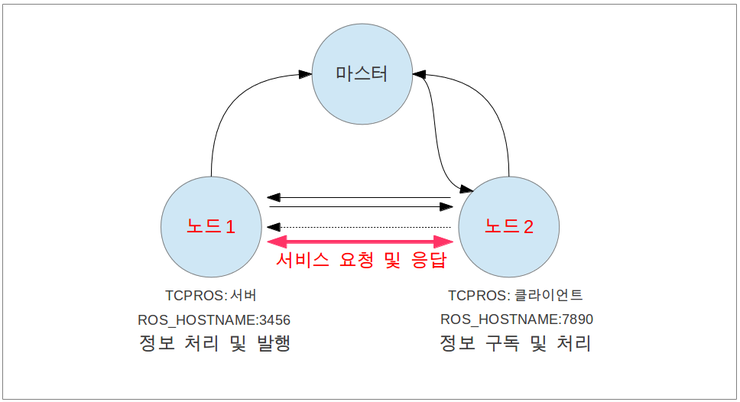
\includegraphics[width=0.6\columnwidth]{pictures/chapter4/notion9.png}
\caption{서비스 요청 및 응답}
\end{figure}

%-------------------------------------------------------------------------------
\subsection{예제}\index{예제}

이전 강좌인 "ROS 강좌 : 07. ROS 동작 테스트" 에서 우리는 "turtlesim"를 이용하여 로스의 구동을 테스트 해보았다. 이 테스트에서도 마스터 및 두 개의 노드가 사용되었고, 두 노드간에는 "/turtle1/cmd\_vel" 라는 토픽을 이용하여 메시지 통신하고 있다. 이를 위해서 설명한 로스 개념 맞추어 생각해보면 다음의 그림처럼 생각할 수 있다.  "ROS 강좌 : 07. ROS 동작 테스트" 의 강좌를 되새김해보며 로스 개념을 다시 한번 생각해 보길 권장한다.

\begin{figure}[h]
\centering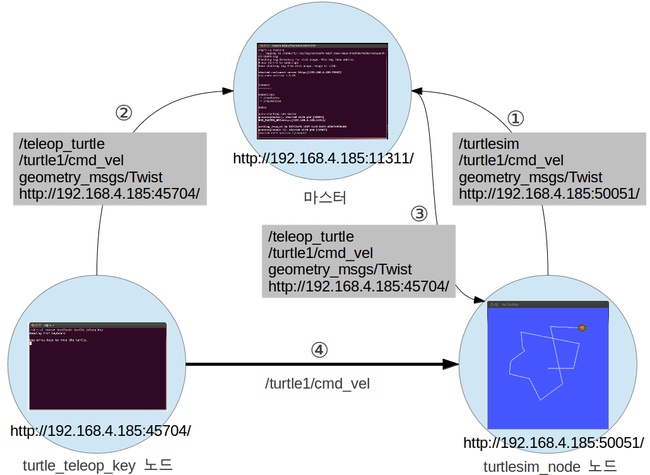
\includegraphics[width=0.6\columnwidth]{pictures/chapter4/notion10.png}
\caption{예제}
\end{figure}

%-------------------------------------------------------------------------------
\section{ROS 파일시스템}\index{ROS 파일시스템}

%-------------------------------------------------------------------------------
\subsection{ROS의 파일 시스템}\index{ROS의 파일 시스템}

로스의 파일 시스템에 대해서 설명하고자 한다. 로스는 크게 "로스 설치 폴더"와 "사용자 작업 폴더"로 구분된다. 

로스 설치 폴더는 로스의 데스크톱 버전을 설치하게 되면 /opt 폴더에 /ros 라는 이름으로 폴더가 생성되고 그 안에 roscore를 포함한 핵심 유틸리티 및 rqt, rviz, 로봇 관련 라이브러리, 시뮬레이션, 네이게이션 등이 설치된다. 사용자는 이 부분의 파일들을 건들일은 거의 없다. 

사용자 작업 폴더는 사용자가 원하는 곳에 폴더를 생성가능한데 필자는 리눅스 사용자 폴더인 "~/catkin\_ws/" (~/ 은 리눅스에서 /home/사용자명에 해당되는 폴더를 의미한다.) 에 설치할 것은 추천한다. 

"로봇 운영체제 강좌 : ROS Indigo 설치" 및 "ROS 강좌 : ROS 개발 환경 구축" 를 진행했다는 가정하에 "로스 설치 폴더"와 "사용자 작업 폴더"에 대한 상세한 내용을 설명하고자 한다.


%-------------------------------------------------------------------------------
\subsection{ROS 설치 폴더}\index{ROS 설치 폴더}

%-------------------------------------------------------------------------------
\subsubsection{설치 경로}\index{설치 경로}

"/opt/ros/[버전명]" 폴더에 설치된다. 예를들어, Indigo 버전을 설치하였을 경우 "/opt/ros/indigo"가 로스 설치 경로이다.

%-------------------------------------------------------------------------------
\subsubsection{파일 구성}\index{파일 구성}

다음의 그림과 같이 "/opt/ros/indigo" 의 폴더아래에 "bin", "etc", "include", "lib", "share" 폴더 및 환경설정 파일들로 구성되어 있다. 

\begin{figure}[h]
\centering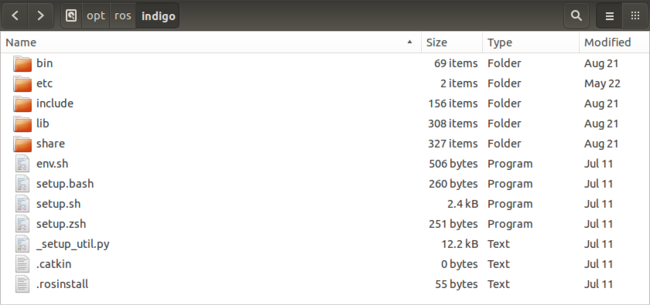
\includegraphics[width=0.5\columnwidth]{pictures/chapter4/folders.png}
\caption{ROS 파일 구성}
\end{figure}

%-------------------------------------------------------------------------------
\subsubsection{세부 내용}\index{세부 내용}

이 폴더에는 로스 설치시에 선택한 패키지를 포함한 로스 구동 제반 프로그램을 포함하고 있다. 세부 내용은 아래와 같다.

\begin{itemize}
\item /bin 실행가능한 바이너리 파일
\item /etc ros 및 catkin 관련 설정파일
\item /include 헤더파일
\item /lib 라이브러리 파일
\item /share ros 패키지
\item env.* 환경설정 파일
\item setup.* 환경설정 파일
\end{itemize}

%-------------------------------------------------------------------------------
\subsection{사용자 작업 폴더}\index{사용자 작업 폴더}

%-------------------------------------------------------------------------------
\subsubsection{사용자 작업 폴더 경로}\index{사용자 작업 폴더 경로}

사용자 작업 폴더는 사용자가 원하는 곳에 폴더를 생성가능하나 강좌의 원활한 진행을 위하여 리눅스 사용자 폴더인 "~/catkin\_ws/" (~/ 은 리눅스에서 /home/사용자명에 해당되는 폴더를 의미한다.) 에 설치할 것은 추천한다. 즉, "/home/사용자명/catkin폴더명"으로 설치하면된다. 예를들어 사용자명이 oroca라는 아이디이고 catkin폴더명은 catkin\_ws라고 설정하였다면 "/home/oroca/catkin\_ws/" 폴더가 된다. 자세한 내용은"로봇 운영체제 강좌 : ROS Indigo 설치" 를 참조하도록 하자. 

%-------------------------------------------------------------------------------
\subsubsection{파일 구성}\index{파일 구성}

다음의 그림과 같이 "/home/사용자명/" 폴더의 아래에 "catkin\_ws" 라는 폴더가 있고, "build", "devel", "src" 폴더로 구성되어 있다. 

\begin{figure}[h]
\centering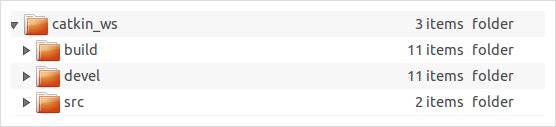
\includegraphics[width=0.5\columnwidth]{pictures/chapter4/folder_catkin_ws.png}
\caption{catkin workspace의 파일 구성}
\end{figure}

%-------------------------------------------------------------------------------
\subsubsection{세부 내용}\index{세부 내용}

이 폴더에는 사용자 작업 폴더로 사용자가 작성한 패키지 및 공개된 다른 개발자의 패키지를 저장하고 빌드하는 공간이다. 사용자는 이 폴더를 작업 폴더로 이용하며 로스 관련된 내부분의 작업을 이 폴더안에서 하게된다. 세부 내용은 아래와 같다.

\begin{itemize}
\item /build catkin 빌드 시스템의 빌드 환경 파일
\item /devel catkin 빌드 시스템에 의해 빌드된 msg, srv 헤더파일 및 사용자 패키지 라이브러리 및 실행파일
\item /src 사용자 패키지
\end{itemize}

%-------------------------------------------------------------------------------
\subsubsection{사용자 패키지}\index{사용자 패키지}

"~/catkin\_ws/src" 폴더에는 사용자가 사용하는 공간이다. 이 폴더에 사용자가 개발한 로스 패키지 및 다른 개발자가 개발한 패키지를 저장하고 빌드하여 실행 파일을 생성해 낼 수 있다. 로스 빌드 시스템은 다음 강좌를 통해 저 자세히 알아 보도록 하고 이번 강좌에는 "이런 폴더와 파일로 구성되어 있구나" 라고 알아두고 넘어가기로 하자. 아래의 예제는 필자가 작성한 "oroca\_ros\_tutorial" 이라는 패키지를 작성한 후의 상태이다. 자세한 내용은 "ROS 강좌 : ROS 빌드 시스템" 및 "메시지 송신 노드와 수신 노드 작성 및 실행"에서 다루어 보기로 하자.

\begin{figure}[h]
\centering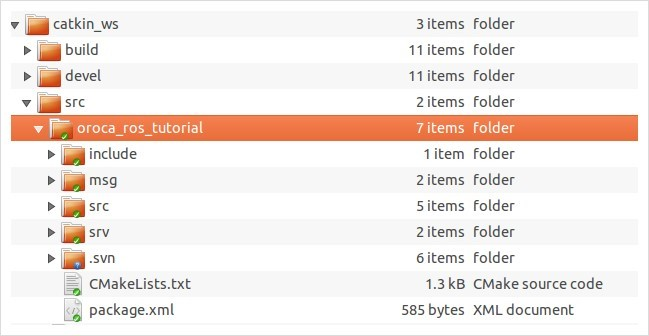
\includegraphics[width=0.5\columnwidth]{pictures/chapter4/folder_oroca_ros_tutorial.jpg}
\caption{사용자 패키지 파일 구성}
\end{figure}

\begin{itemize}
\item /include 헤더파일
\item /launch 로스런치에 사용되는 스크립트
\item /node rospy용 스크립트
\item /msg 메시지 파일
\item /src 코드 소스 파일
\item /srv 서비스 파일
\item CMakeLists.txt 빌드 설정 파일
\item package.xml 패키지 설정 파일
\end{itemize}

%-------------------------------------------------------------------------------
\section{ROS 빌드 시스템}\index{ROS 빌드 시스템}

%-------------------------------------------------------------------------------
\subsection{ROS 빌드 시스템}\index{ROS 빌드 시스템}

로스의 빌드 시스템은 기본적으로 CMake(Cross Platform Make)\footnote{CMake, wikipedia, http://ko.wikipedia.org/wiki/CMake} 를 이용하고 있고, 패키지 폴더에 CMakeLists.txt 라는 파일에 빌드 환경을 기술하고 있다. 로스에서는 CMake를 로스에 맞도록 수정하여 로스에 특화된 캐킨 빌드 시스템을 만들었다. 

로스에서 CMake를 이용하고 있는 이유는 멀티플랫폼에서 로스 패키지를 빌드할 수 있도록 위함이다. Make\footnote{Make, wikipedia, http://ko.wikipedia.org/wiki/Make}가 유닉스계열만 지원하는 것과 달리, CMake는 유닉스 계열인 리눅스, BSD, OS X 뿐만 아니라 윈도우 계열도 지원하기 때문이다. 또한, 마이크로소프트 비주얼 스튜디오도 지원하고 QT개발에도 쉽게 적용될 수 있다. 

더욱이, 캐킨 빌드 시스템은 로스와 관련된 빌드, 패키지 관리, 패키지간의 의존관계 등을 편리하게 사용할 수 있도록 하고 있다. 

%-------------------------------------------------------------------------------
\subsection{패키지 생성}\index{패키지 생성}

로스 패키지를 생성하기 위해서는 다음과 같은 명령어를 이용한다. "catkin\_create\_pkg" 는 사용자가 패키지를 작성할때 캐킨 빌드 시스템에 꼭 필요한 CMakeLists.txt 와 package.xml 를 포함한 패키지 폴더를 생성한다. 실제로 간단한 패키지를 작성해 보자.

\begin{lstlisting}[language=bash]
catkin_create_pkg %*[패키지이름] [의존하는패키지1] [의존하는패키지2] [의존하는패키지3]*)
\end{lstlisting}

%-------------------------------------------------------------------------------
\subsubsection{작업 폴더로 이동}\index{작업 폴더로 이동}

\begin{lstlisting}[language=bash]
$ cd ~/catkin_ws/src
\end{lstlisting}

%-------------------------------------------------------------------------------
\subsubsection{패키지 생성}\index{패키지 생성}

"my\_first\_ros\_pkg" 라는 이름의 패키지를 생성할 것이다. 

로스에서는 패키지 이름에는 모두 소문자를 사용하며, 스페이스바와 같은 공백이 있으면 안된다. 그리고 일반적으로 하이픈(-) 대신에 밑줄(\_)을 사용하여 각 단어를 이어붙이는 것을 관례로 하고 있다. 

그리고 이번에는 의존하는 패키지로 "std\_msgs"와 "roscpp"를 옵션으로 달아주었다. 로스의 표준 메시지 패키지인 std\_msgs 와 로스에서 C/C++을 사용하기 위하여 클라이언트라이브러인 roscpp를 사용하겠다는 것으로 패키지 생성에 앞어서 미리 설치해야한다는 의미이다. 이러한 의존하는 패키지의 설정은 패키지 생성할 때 지정할 수도 있지만, 생성 후 package.xml 에서 직접 입력하여도 된다.

\begin{lstlisting}[language=bash]
$ catkin_create_pkg my_first_ros_pkg std_msgs roscpp
\end{lstlisting}

위와 같이 패키지를 생성하였으면 "~/catkin\_ws/src"에 "my\_first\_ros\_pkg" 라는 패키지 폴더 및 로스 패키지가 갖추어야할 기본 내부 폴더 및 CMakeLists.txt 와 package.xml가 생성된다. 다음과 같이 명령어로 ls 를 입력하여 내용을 보던가 윈도우의 탐색기와 같은 역할을 하는 GUI기반의 Nautilus를 이용하여 패키지 내부를 살펴보도록 하자.

\begin{lstlisting}[language=bash]
$ ls
include       %*.......... 인클루드 폴더*)
src           %*.......... 소스코드 폴더*)
CMakeLists.txt%*.......... 빌드 설정 파일*)
package.xml   %*.......... 패키지 설정 파일*)
\end{lstlisting}

\begin{figure}[h]
\centering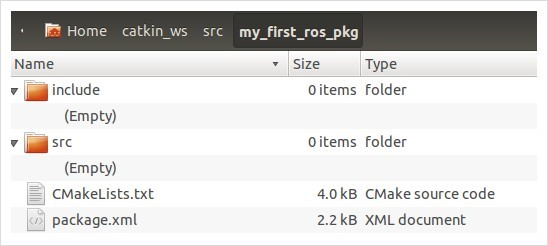
\includegraphics[width=0.5\columnwidth]{pictures/chapter4/new_package.jpg}
\caption{caption}
\end{figure}

%-------------------------------------------------------------------------------
\subsection{패키지 설정 파일 (package.xml) 수정}\index{패키지 설정 파일 (package.xml) 수정}

로스의 필수 설정 파일 중 하나인 package.xml 은 패키지의 정보를 담은 XML 파일로써 패키지의 이름, 저작자, 라이선스, 의존성 패키지 등을 기술하고 있다. 처음에 아무런 수정을 가하지 않은 원본 파일은 다음과 같다.

\lstinputlisting[language=XML, numbers=none, caption=package.xml]{./sources/package.xml}

\begin{itemize}
\item \textless{?xml}\textgreater 문서 분법을 정의하는 문구로 아래의 내용은 xml 버전 1.0을 따르고 있다는 것을 알리고 있다.
\item \textless{package}\textgreater 이 구문부터 \textless/package\textgreater 까지가 로스 패키지 설정 부분이다.
\item \textless{name}\textgreater 패키지의 이름이다. 패키지 생성할때 입력한 패키지 이름이 사용된다. 다른 옵션도 마찬가지이지만 이는 사용자가 원할때 언제든지 변경할 수 있다.
\item \textless{version}\textgreater 패키지의 버전이다. 자유롭게 지정할 수 있다.
\item \textless{description}\textgreater 패키지의 간단한 설명이다. 
\item \textless{maintainer}\textgreater 패키지 관리자의 연락처를 기재한다.
\item \textless{license}\textgreater 라이선스를 기재한다. BSD, MIT, GPLv3, LGPLv3 등을 기재하면 된다. 오로카에서는 MIT를 사용하고 있다.
\item \textless{url}\textgreater 패키지를 설명하는 웹 페이지 또는 버그관리, 저장소 등의 주소를 기입한다. 이 종류에 따라 type에  website, bugtracker, repository 를 대입하면 된다. 참고로 url 태그는 옵션이다.
\item \textless{author}\textgreater 패키지 개발에 참여한 개발자를 적어주면 된다. 참고로 author 태그는 옵션이다.
\item \textless{buildtool\_depend}\textgreater 빌드 시스템의 의존성을 기술한다. 지금은 캐킨 빌드 시스템을 이용하고 있기 때문에 catkin 를 입력하면 된다.
\item \textless{build\_depend}\textgreater 패키지를 빌드할 때 의존하는 패키지명을 적어준다.
\item \textless{run\_depend}\textgreater 패키지를 실행할 때 의존하는 패키지명을 적어준다.
\item \textless{test\_depend}\textgreater 패키지를 테스트할때 의존하는 패키지명을 적어준다. 테스트이외에는 사용하지 않는다.
\item \textless{export}\textgreater 로스에서 명시하지 않은 태그명을 사용할때 쓰인다. 일반적인 경우 쓸일이 없다.
\item \textless{metapackage/}\textgreater export 태그 안에서 사용하는 공식적인 태그로 현재의 패키지가 메타패키지의 경우 이를 선언한다.
\end{itemize}

\noindent
필자는 다음과 같이 패키지 설정 파일(package.xml)을 수정하였다. 여러분은 자신에 맞게 수정해보도록 하자.

\begin{lstlisting}[language=XML]
<?xml version="1.0"?>
<package>
  <name>my_first_ros_pkg</name>
  <version>0.0.1</version>
  <description>The my_first_ros_pkg package</description>
 
  <maintainer email="passionvirus@gmail.com">Yoonseok Pyo</maintainer>
  <license>MIT</license>
  <url type="website">http://cafe.naver.com/openrt/2500</url>
  <url type="repository">https://github.com/oroca/oroca_ros_tutorials.git</url>
  <author email="passionvirus@gmail.com">Yoonseok Pyo</author>
 
  <buildtool_depend>catkin</buildtool_depend>
 
  <build_depend>std_msgs</build_depend>
  <build_depend>roscpp</build_depend>
 
  <run_depend>std_msgs</run_depend>
  <run_depend>roscpp</run_depend>
 
  <export>
  </export>
</package>
\end{lstlisting}

%-------------------------------------------------------------------------------
\subsection{빌드 설정 파일 (CMakeLists.txt) 수정}\index{빌드 설정 파일 (CMakeLists.txt) 수정}

로스의 빌드 시스템인 캐킨은 기본적으로 CMake를 이용하고 있어서 패키지 폴더에 CMakeLists.txt 라는 파일에 빌드 환경을 기술하고 있다. 이는 실행 파일 생성, 의존성 패키지 우선 빌드, 링크 생성 등을 설정하게 되어 있다. 처음에 아무런 수정을 가하지 않은 원본 파일은 다음과 같다.

\lstinputlisting[language=make, numbers=none, caption=CMakeLists.txt]{./sources/CMakeLists.txt}

\noindent
빌드 설정 파일 (CMakeLists.txt)의 각 옵션들은 다음과 같다.

\begin{lstlisting}[language=make,backgroundcolor=\color{white}]
// %*운영체제에 설치되어 있는 cmake의 최소한의 버전이다. 현재에는 2.8.3 버전으로 명시되어 있다. 이 보다 낮은 cmake를 사용하는 경우에는 버전 업데이트를 해줘야 한다.*)
cmake_minimum_required(VERSION 2.8.3)

// %*패키지의 이름이다. package.xml 에서 입력한 패키지 이름을 그대로 사용하자.*)
project(my_first_ros_pkg)

// %*캐킨 빌드를 할 때 요구되는 구성요소 패키지이다. 현재 의존성 패키지로 roscpp 및 std\_msgs가 추가되어 있다. 여기에 입력된 패키지가 없는 경우 캐킨 빌드할 때 사용자에게 에러가 표시된다. 즉, 사용자가 만든 패키지가 의존하는 패키지를 먼저 설치하게 만드는 옵션이다.*)
find_package(catkin REQUIRED COMPONENTS
  roscpp
  std_msgs
)

// %*로스 이외의 패키지를 사용하는 경우에 사용되는 방법이다. 예를들어 다음의 경우, Boost를 사용할때 system 이라는 패키지가 설되어 있어야 한다. 기능은 위에서 설명한 의존하는 패키지를 먼저 설치하게 만드는 옵션이다.*)
find_package(Boost REQUIRED COMPONENTS system)

// %*파이썬을 사용할 때 설정하는 옵션이다. 파이썬은 cmake를 사용할 필요없는 스크립트 언어이지만 패키지의 호환성을 위해 아래와 같이 독자적인 설정을 하게 되어 있다.*)
catkin_python_setup()

// %*사용하는 메시지 파일을 추가하는 옵션이다. FILES를 사용하면 패키지 폴더의 "msg" 안의 .msg 파일들을 참조하게 된다. 다음의 예제에서는 Message1.msg 및 Message2.msg 의 메시지 파일을 이용하겠다는 옵션이다.*)
add_message_files(
  FILES
  Message1.msg
  Message2.msg
)

// %*사용하는 서비스 파일을 추가하는 옵션이다. FILES를 사용하면 패키지 폴더의 "srv" 안의 .srv 파일들을 참조하게 된다. 다음의 예제에서는 Service1.srv 및 Service2.srv 의 서비스 파일을 이용하겠다는 옵션이다.*)
add_service_files(
  FILES
  Service1.srv
  Service2.srv
)

// %*의존하는 메시지를 사용하겠다는 옵션이다. 다음의 예제에서는 DEPENDENCIES 옵션에 의하여 std\_msgs 라는 메시지 패키지를 사용하겠다는 설정이다.*)
generate_messages(
  DEPENDENCIES
  std_msgs
)

// %*캐킨 빌드 옵션이다.*)
// %*"INCLUDE\_DIRS"는 뒤에 설정한 패키지 내부 폴더인 "include"의 헤더파일을 사용하겠다는 설정이다.*)
// %*"LIBRARIES"는 뒤에 설정한 패키지의 라이브러리를 사용하겠다는 설정이다.*)
// %*"CATKIN\_DEPENDS" 캐킨 빌드할 때 의존하는 패키지들이다. 현재  roscpp 및 std\_msgs가 의존하고 있다는 설정이다.*)
// %*"DEPENDS" 시스템 의존 패키지를 기술하는 설정이다.*)
catkin_package(
 INCLUDE_DIRS include
 LIBRARIES my_first_ros_pkg
 CATKIN_DEPENDS roscpp std_msgs
 DEPENDS system_lib
)

// %*인클루드 폴더를 지정할 수 있는 옵션이다. 현재 \$\{catkin\_INCLUDE\_DIRS\} 라고 설정되어 있는데 이는 각 패키지안의 "include" 폴더를 의미하고 이 안의 헤더파일을 이용 하겠다는 설정이다.*)
include_directories(
  ${catkin_INCLUDE_DIRS}
)

// %*cpp 라이브러리를 선언한다. src/\$\{PROJECT\_NAME\}/my\_first\_ros\_pkg.cpp 파일을 참조하여 my\_first\_ros\_pkg 라는 라이브러리를 생성하게 된다.*)
add_library(my_first_ros_pkg
  src/\${PROJECT_NAME}/my_first_ros_pkg.cpp
)

// %*cpp 실행 파일을 선언한다. src/my\_first\_ros\_pkg\_node.cpp 파일을 참조하여 my\_first\_ros\_pkg\_node 라는 실행파일을 생성한다.*)
add_executable(my_first_ros_pkg_node src/my_first_ros_pkg_node.cpp)

// %*패키지를 빌드하기 앞서서 생성해야할 메시지 헤더파일이 있을 경우 빌드전에 우선적으로 메시지를 생성하라는 설정이다. 현재 my\_first\_ros\_pkg\_generate\_messages\_cpp 를 우선적으로 빌드하고 my\_first\_ros\_pkg\_node 를 빌드하게 하는 설정이다.*)
add_dependencies(my_first_ros_pkg_node my_first_ros_pkg_generate_messages_cpp)

// %*my\_first\_ros\_pkg\_node 를 생성하기 앞서서 링크해야하는 라이브러리 및 실행파일을 링크해주는 옵션이다.*)
target_link_libraries(my_first_ros_pkg_node
  \${catkin_LIBRARIES}
)
\end{lstlisting}

\noindent
필자는 다음과 같이 빌드 설정 파일(CMakelists.txt)을 수정하였다. 여러분은 자신에 맞게 수정해보도록 하자.

\begin{lstlisting}[language=make]
cmake_minimum_required(VERSION 2.8.3)
project(my_first_ros_pkg)
 
find_package(catkin REQUIRED COMPONENTS
  roscpp
  std_msgs
)
 
catkin_package(
  INCLUDE_DIRS include
  CATKIN_DEPENDS roscpp std_msgs
  DEPENDS system_lib
)
 
include_directories(
  ${catkin_INCLUDE_DIRS}
)
 
add_executable(hello_world_node src/hello_world_node.cpp)
add_dependencies(hello_world_node my_first_ros_pkg_generate_messages_cpp)
target_link_libraries(hello_world_node ${catkin_LIBRARIES})
\end{lstlisting}

%-------------------------------------------------------------------------------
\subsection{소스코드 작성}\index{소스코드 작성}

위에서 필자가 작성한 CMakelists.txt 파일을 참고하길 바란다. 실행파일 생성 부분에서 다음과 같이 설정해 놓았다. 즉, 패키지의 "src" 폴더에 있는 "hello\_world\_node.cpp" 소스코드를 참고하여 "hello\_world\_node" 라는 실행파일을 생성하라는 설정이다. 여기서, "hello\_world\_node.cpp" 소스코드가 없기에 간단한 예제로 하나 작성해 보자. 다음의 예제에서는 nano라는 에디터를 사용하였으나 vi, gedit, qtcreator 등 자신이 원하는 편집기를 이용하면 된다.

\noindent
"add\_executable(hello\_world\_node src/hello\_world\_node.cpp)"

\begin{lstlisting}[language=bash]
$ cd /src     %* //여기서 src 는 자신의 패키지 폴더안의 src 라는 소스코드를 담는 폴더를 말한다.*)
$ nano hello_world_node.cpp
\end{lstlisting}

\begin{lstlisting}[language=C++]
#include <ros/ros.h>
#include <std_msgs/String.h>

#include <sstream>

int main(int argc, char **argv)
{
  ros::init(argc, argv, "hello_world_node");
  ros::NodeHandle nh;
  ros::Publisher chatter_pub = nh.advertise<std_msgs::String>("say_hello_world", 1000);

  ros::Rate loop_rate(10);
  int count = 0;
  while (ros::ok())
  {
    std_msgs::String msg;
    std::stringstream ss;
    ss << "hello world " << count;
    msg.data = ss.str();
    ROS_INFO("%s", msg.data.c_str());
    chatter_pub.publish(msg);
    ros::spinOnce();
    loop_rate.sleep();
    ++count;
  }
  return 0;
}
\end{lstlisting}

%-------------------------------------------------------------------------------
\subsection{패키지 빌드}\index{패키지 빌드}

이제 패키지 빌드를 위한 모든 작업이 완료되었다.  빌드에 앞서서 다음의 명령어로 로스 패키지의 프로파일을 갱신시켜주자. 앞서 제작한 우리의 패키지를 로스 패키지 목록에 반영시켜주는 명령어이다. 필수 사항은 아니지만 새로 패키지를 생성한 후에 갱신해주면 이용하기 편하다.

\begin{lstlisting}[language=bash]
$ rospack profile
\end{lstlisting}

\noindent
다음은 캐킨 빌드 이다. 캐킨 작업 폴더로 이용하여 캐킨 빌드를 해주자.

\begin{lstlisting}[language=bash]
$ cd ~/catkin_ws && catkin_make
%*또는*)
$ cm
\end{lstlisting}

\noindent
이전 강좌인 "ROS 강좌 : 06. ROS 개발 환경 구축"에서 언급했듯이 .bashrc 파일에 alias \verb|cm='cd ~/catkin_ws && catkin_make'| 라고 설정해두면 터미널 창에서 "cm" 이라는 간단한 명령어로 위의 명령어를 대체할 수 있다. 유용한 만큼 이전 강좌를 보고 꼭 설정해 두도록 하자.

%-------------------------------------------------------------------------------
\subsection{노드 실행}\index{노드 실행}

에러 없이 빌드가 완료되었으면 "~/catkin\_ws/devel/lib/my\_first\_ros\_pkg" 에 "hello\_world\_node" 라는 파일이 생성되었을 것이다. 한번 확인해 보자.

다음 단계는 노드를 실행하는 것인데 노드 실행에 앞서서 roscore를 구동하자. 로스의 모든 노드는 roscore를 구동한 후에 이용할 수 있다.

\begin{lstlisting}[language=bash]
$ roscore
\end{lstlisting}

\noindent
마지막으로 새로운 터미널창을 열어 아래의 명령어로 노드를 실행해보자. my\_first\_ros\_pkg 라는 패키지의 hello\_world\_node 라는 노드를 실행하라는 명령어이다.

\begin{lstlisting}[language=bash]
$ rosrun my_first_ros_pkg hello_world_node 
[ INFO] [1380598894.131775283]: hello world 0
[ INFO] [1380598894.231826916]: hello world 1
[ INFO] [1380598894.331798085]: hello world 2
[ INFO] [1380598894.431796634]: hello world 3
[ INFO] [1380598894.531808660]: hello world 4
[ INFO] [1380598894.631800431]: hello world 5
[ INFO] [1380598894.731805683]: hello world 6
\end{lstlisting}

\noindent
노드를 실행하게 되면 위와 같이 hello world 1, 2 ,3 과 같은 메시지가 발행되는 것을 볼 수 있을 것이다. 이번 강좌는 로스의 빌드 시스템을 설명하기 위한 것이니 노드의 소스코드에 관해서는 다음 강좌를 통해 알아보도록 하자.


%-------------------------------------------------------------------------------